\documentclass{article}

\usepackage{cite}
\usepackage{listings}
\usepackage{times}
\usepackage{color}
\usepackage{url}
\usepackage{multirow}
\usepackage{enumitem} % Use for enumerating A, B, C etc...
\urlstyle{same} % Used for formatting formatting url footnotes
\usepackage{amsmath} % Used in some math formulas

\usepackage[table]{xcolor}% http://ctan.org/pkg/xcolor
\usepackage{soul} % highlighting

%\usepackage[top=.3in, bottom=1in, left=1in, right=1in]{geometry} %% Changes the margins of the pages
\usepackage[bottom=1in, left=1in, right=1in, top=1in]{geometry} 

\usepackage{pgfgantt} % ALso helps with images

\newcommand{\todo}[1]{\textcolor{cyan}{\textbf{[#1]}}}
\newcommand{\dan}[1]{\textcolor{blue}{{\it [Dan says: #1]}}}
\newcommand{\qi}[1]{\textcolor{red}{{\it [Qi says: #1]}}}

% Addressing Decision-Making Uncertainty in Intelligent Systems By Accounting for Tactic Volatility
% Reducing Tactic Uncertainty in Intelligent Systems

% Addressing Tactic Volatility in Intelligent Systems
% Reducing Tactic Uncertainty in Intelligent Systems to Make More Informed Decisions

\newcommand{\Title}{Reducing Tactic Uncertainty in Self-Adaptive Systems}
\newcommand{\CallNumber}{XXXXX}

% Clean up the title a bit

% DK: Give it a better name since reviewers will likely respond with "what is new about addressing decision-making uncertainty" - Need to make it clear early on that this is a new area

\usepackage{fancyhdr} % Header
\pagestyle{fancy}
\lhead{\CallNumber} % Leave empty to keep sections from being shown
\rhead{\Title}


\usepackage{lastpage}
\cfoot{\thepage\ of \pageref{LastPage}}
\begin{document}

\begin{titlepage}

  \newcommand{\HRule}{\rule{\linewidth}{0.5mm}} % Defines a new command for the horizontal lines, change thickness here

  \center % Center everything on the page


%	HEADING SECTION

  %\textsc{\LARGE University Name}\\[1.5cm] % Name of your university/college
  \textsc{\Large White Paper Submission}\\[0.5cm] % Major heading such as course name
  \textsc{\large \CallNumber}\\[0.5cm]   %% Name of Call
  
  % ONR BAA: N00014-18-S-B001
  % AFRL BAA: 
  % ARL BAA: 

%	TITLE SECTION





 \vspace{1.5 cm}
  \HRule \\[0.4cm]
  { \huge \bfseries \Title}\\[0.4cm] % Title of your document
  \HRule \\[1.5cm]
 
  \vspace{.5 cm}
   Qi Yu and Daniel E. Krutz\\
  Rochester Institute of Technology\\
 %  \vspace{.5 cm}
% GOL-1575\\
 134 Lomb Memorial Drive\\
 Rochester, NY 14623\\
 %1 (585) 475 2896\\
 \{qyuvks, dxkvse\}@rit.edu\\

%	DATE SECTION

  \vspace{1.5 cm}
  {\large Submitted: \today}\\[3cm] % Date, change the \today to a set date if you want to be precise


\vfill % Fill the rest of the page with whitespace

\end{titlepage}




%\maketitle
%\centerline{\large\bf \Title} % Was "Large"

%% Maybe just have a 2-3 sentence overview
%\section{Overview}


\section{Statement of the Work}
% Include a statement of work (SOW) concisely detailing the scope and objectives of the effort and the technical approach. It should be limited to half a page.

\textbf{This proposal will demonstrate the detrimental effects of not properly accounting for decision (tactic) volatility in self-adaptive systems, and will create and evaluate methods for accounting for tactic uncertainty in the decision-making process.} We will accomplish this through statistical simulations and modeling, the use of existing and to be created simulation tools, and through implementation in physical devices such as UAVs.

%% Add in something about uncertainty reduction?

%Uncertainty comes from many sources. For example, can you trust the system's users? Can you trust their data ? (Has it been checked to make sure that it is ok)

\section{Problem Statement}
As human beings, we rely upon accurate information to make appropriate decisions. Using inaccurate data often leads to improper decisions. Autonomous systems act similarly. Autonomous systems rely upon accurate information to make decisions that lead to the maximum utility (benefit). Inaccurate information used in the decision-making process will often lead to decisions leading  to less than optimal utility. \emph{Uncertainty} inherently exists in many types of self-adaptation environments. Fortunately, many adaptation processes are beginning to account for uncertainty. However, no decision-making processes properly account for tactic (decision) uncertainty during the adaptation process. This includes tactic latency uncertainty, tactic reliability uncertainty, and possible volatility of the utility generated by the individual tactic. Uncertainty in autonomous has been shown to have detrimental effects on the resiliency and dependability of the system.%\todo{cite}. %? Should I even say more?

%This may affect the system's ability to properly complete all mission objectives. In a military UAV for example\hl{...}



% In this section the principal investigator answers the question, “What is the system-level problem to be solved and why is it important?” It need only be a paragraph stating the problem and the possible military benefit (new or improved capability) if a solution is found. Half a page should be sufficient. 



% Include a motivating example somewhere in the paper


\section{Technical Background}

%This section provides the broader context in which the white paper is being submitted, providing an elaboration of the problem statement and military benefits stated in the previous section (Problem Statement). It may include a historical overview of the problem with respect to a current system capability performance shortfall, previous approaches to solving the problem that either provided the current capability or failed to provide a needed capability, and a brief explanation of any current line of research that promises a solution. This section may require more than one page. References should be cited if they can provide additional background. Of particular value are reports describing test and evaluation (T&E) trials of developing or in-fleet systems that document a specific system performance shortfall, or a concept-of-operations study that quantifies the gain from a hypothesized new system or an improved capability in an existing system. 


To provide the appropriate technical background for our proposed work, we will begin by describing \emph{tactics} (decisions) and \emph{uncertainty} in intelligent systems.

\paragraph{Tactics (Decisions)}Self-adaptive systems (SAS) have the ability to alter their configuration and/or functionality to react to changing internal or external events while continuing to fulfill system requirements and maximizing the utility (benefit) of the system~\cite{moreno2017decision}. A challenging decision for these systems is when and how they should react to a nearly infinite number of possible scenarios. Decision-making processes frequently use \emph{tactics} to alter the structure or system properties to respond to these changing situations~\cite{moreno2017adaptation}. An example tactic could be provisioning a virtual machine in a web farm when the workload is about to reach a specific threshold, or activating the deicing mechanism on a UAV when defined environmental conditions are encountered.


%% Might want to address this depending on where we go with the paper
%\vspace{3mm} \noindent \textbf{Uncertainty}
\paragraph{Uncertainty}Some examples of uncertainty include the precise actions a human may take with a system, how an adversary may attempt to compromise a UAV, or even possible component failures. Uncertainty can be grouped into internal or external categories. An example of external uncertainty for a UAV could be weather conditions. An example of internal uncertainty is determining the impact of an adaptation decision on the quality attributes of a system. Such an event could be determining the impact of replacing a software component to the system's responsiveness, or even on battery usage. As with humans, self-adaptive systems need accurate information to make well-informed decisions. Uncertainty has been shown to affect numerous areas of a self-adaptive system ranging from its decision-making effectiveness and efficiency, leading to directly impact the system's resiliency, robustness and ability to complete all mission objectives~\cite{mahdavi2016classification, camara2017uncertainty}. Despite the well-deserved emphasis uncertainty has been gaining, to our knowledge it has not been properly addressed from a tactic perspective. Some examples of tactic uncertainties include:


% DK: For the full proposal these should be expanded upon quite a bit with diagrams and more citations

\begin{enumerate}[noitemsep]
	\item \textbf{Tactic Latency} The amount of time required to implement a decision (tactic) is known as \emph{Tactic latency}. For example, the time required to activate a virtual machine in a cloud environment would be the tactic latency. This latency value typically varies between different tactics. For example, the time required to prepare a UAV for landing will likely be very different from the time required to perform a simple calculation. The latency of each tactic has a significant impact on the decisions made by the system. When multiple tactics may be used to address a specific situation, the tactic with the maximum utility should be selected by the system, and this latency is often a determining factor. Previous works have shown that latency aware algorithms offer several advantages compared to those that do not consider latency~\cite{camara2014stochastic, esfahani2013learning}. Due to the unpredictable nature of many tactics, their latency cannot always be predicted. Unfortunately, existing decision-making processes that do account for tactic latency all consider it to be a predetermined, static value. When a system is not able to account for tactic latency or `learn' about what this value should be expected to be, then this creates unnecessary uncertainty in the system.
    
    
	\item \textbf{Tactic Dependability} 
    % Explain how tactic dependability and tactic availability are different

The measure how how well a tactic correctly produces its expected functionality is known as \emph{Tactic Dependability}. Due to numerous reasons, tactics can sometimes fail to produce the expected results. For example, a tactic to perform a calculation could return a inaccurate result, or a virtual machine could fail to properly activate. Knowing when a tactic is not working dependability is imperative for an autonomous system. For example, if a system has two tactic options and it chooses the option with a slightly higher utility, but high failure rate; then the system could frequently waste its time trying to implement a tactic that frequently fails, but only returns slightly better benefit than its more reliable alternative.


%Knowing when a tactic is not working dependability is imperative for an autonomous system. For example if a UAV is deciding on two options and one may typically have higher benefit than the other, but has been shown to not be dependable, then this should be accounted for in the decision-making process. While knowing a tactic has failed may be challenging and the verification method may be highly dependent on the specific tactic, \emph{assurance cases} have been shown to provide a reliable method of knowing if a tactic performed properly.





%While assurance cases can help identify points of failure, they are not inherently included in the decision-making process\dan{Is this true? Check this}.
   


    
    
    
    
    
    
     
    
%%%%%%    <-- This may be useful for full paper proposals
%    Tactics come in many shapes and forms. Tactics may be in the form of performing a simple calculation, activating a virtual machine, or even firing a missile. Due to numerous reasons, tactics may fail. For example, a network connection may periodically fail meaning the tactic is unavailable. In a UAV, the deicer may not be properly functioning on a specific mission. Current decision-making systems do not consider tactic dependability in their decision-making process. While assurance cases can help identify points of failure, they are not inherently included in the decision-making process\dan{Is this true? Check this}.


%An existing problem with not accounting for tactic unavailability is that systems are unable to learn from previous tactic availability experiences and include this in the decision-making process. Due to this inability to learn, the system may continue to make the same mistake over and over. For example, consider a system with two tactic options, with option $A$ returning a slightly larger utility benefit than option $B$. However, in previous events, tactic $A$ has been found to have a high rate of failure. This high rate of failure should be accounted for in the decision-making process and \todo{finish this}


%Knowing when a tactic is not working dependability is imperative for an autonomous system. For example if a UAV is deciding on two options and one may typically have higher benefit than the other, but has been shown to not be dependable, then this should be accounted for in the decision-making process. While knowing a tactic has failed may be challenging and the verification method may be highly dependent on the specific tactic, \emph{assurance cases} have been shown to provide a reliable method of knowing if a tactic performed properly.

%-- The tactic may only return part of the initially defined benefit



\item \textbf{Tactic Availability} For various reasons, tactics may sometimes be unavailable. For example, one tactic may be to retrieve information from a remote server, but the connection to this server may be unreliable. The system should be able to understand the likelihood of this unavailability and consider it in the decision-making process. For example, if the system has observed that this connection was unavailable in 20\% of the previous attempts, then it should consider this success rate before making future attempts. 

The detrimental effects of not being able to learn from the failure rate could be significant and include I) Lost time due to the system trying a tactic that didn't work. This could also affect concurrent and subsequent tactic decisions. II) Potentially lost energy from attempting tactic with a high failure rate. In devices such as UAVs, power is of paramount importance, and attempting a tactic that is fails could cost the system significant amounts of precious energy.


The idea of tactic dependability and tactic availability differ in that tactic dependability refers to a tactic's ability to produce the expected results, while tactic availability is when the tactic is an available option when called option. % Move this?


%An existing problem with not accounting for tactic unavailability is that since system's are unable to learn from previous availability experiences in the decision-making process, this could lead to them repeating problems over and over. For example, consider a system that has two possible decisions, with option $A$ returning a slightly benefit utility than option $B$. 






%The system should be able to account for this potential unavab




% Another server is not available


% Ping 


% Trying a tactic that is not available could cost time, affecting the system's resiliency. For example....







% Maybe move this up
%	\item \textbf{Tactic Utility} An objective of intelligent systems is to make decisions that lead to the most utility (benefit). \dan{Jeff: Should we include this?}

% What may be good one minute has less benefits the next


	% Component dependability 
	% Consider assurance cases of the tactic back into the decision-making process (has this been done before)
    % Tactic trustworthiness?
    % Tactic "Cost" (User impact etc.... -> Not sure where I am going with this)
	% Human uncertainty

\end{enumerate}




% In full proposal maybe provide a cloud-based example as well if space allows
%	In NSF proposal we should also discuss the need to create a simulator
% \vspace{3mm} \noindent 
\paragraph{Motivating Example} To demonstrate the need for accounting for tactic volatility during the decision-making process, we will describe the following motivating UAV example. In our example, a military UAV is flying in a hostile environment. One tactic is to prepare missiles for launch when a target is identified. In a scenario where the UAV identities a possible target, several steps must be taken. In this example, we will assume that the UAV needs to physically prep the missile for launch (planned time of 2 seconds), and will need to communicate with the base station to confirm the target and perform other necessary calculations (planned time of 4 seconds). This anticipated latency time means that the UAV should plan on beginning the target engagement process 4 seconds before it is in range. However, in the event of tactic latency volatility, perhaps due to weather conditions, it could take 6 seconds to communicate with the base station and receive the required data. Not accounting for this latency volatility could lead to a less an optimal decision, one where the UAV was past its target. If the UAV was able to use knowledge about its prior mission experiences about lag with communicating with the base station, it would be able to account for this expected lag in its future decisions. By enabling the UAV to account for tactic latency volatility and include this in its decision-making process, the UAV will be able to make a more informed decision likely enabling it to complete all mission objectives more successfully. This example scenario is shown in Figure~\ref{fig:UAVLatencyExample}. 

\begin{figure}[h]
	\centering
    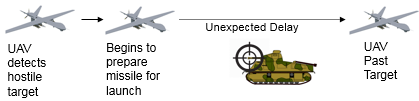
\includegraphics[scale=0.7]{images/UAVLatencyExample.png}
    \caption{Impact of Unexpected Latency in UAV}
    \label{fig:UAVLatencyExample}
\end{figure}

% Talk about how it leads to uncertainty



%To demonstrate the need for accounting for tactic uncertainty during the decision-making process, we will describe the following motivating UAV example. A military UAV is operating autonomously and identifies a possible target. In this scenario, we will assume that the UAV needs to communicate with the base station to receive automatically generated information that is used to determine if the target should be engaged or not. The anticipated time required to make this decision has a significant impact on the actions of the UAV. In current decision-making systems that consider tactic latency, they all determine the required determination time to be a static, pre-defined value. However, in the case of this UAV it can be assumed to be a volatile value, one that represents uncertainty. For example, the communication and determination time could be impacted by weather influenced factors, adversaries jamming the communication, or merely due to unforeseen computation and response time from the base station. In our example, since the decision-making process is unable to account for this volatility and uncertainty in the decision-making process, it could then lead to the UAV flying past the target before a decision can be reached. Since the tactic latency time is considered to be a static value, uncertainty exists over what the actual latency time.  \dan{clean all of this up}


% An overview of this motivating example is shown in Figure~\ref{fig:motivatingExample}.


% \begin{figure}[h]
% 	\centering
%     
\includegraphics[scale=0.4]{images/dummy.png}
%     \caption{XXXX}
%     \label{fig:motivatingExample}
% \end{figure}



%Based on it's speed and\todo{finish this} 


%% Preparing missle for launch
%	two possible tatcics: 
%	Engage target and slow down to hit target

% Base station communications take longer than expected, miss target opportunity
% 


% Might be a good idea to include an image here



%To demonstrate 

%Due to many of the self-adaptive systems in the world being military related, whether it be UAV's or submarines etc., our proposed LVA technique is driven by mission-critical systems. For example, UAV's are often the go-to system for military surveillance purposes as they can be remotely controlled from a base that's thousands of miles from where it is flying, or it can be programmed with a mission to fly on its own and not return to base until the mission has been completed. When the UAV is flying on its own like this, i.e. autopilot, it is \textit{critical} that the system has the capability to adapt to its surrounding environment, without putting the mission or the UAV itself, at risk. The following diagram represents a scenario in which a UAV that has been programmed to fly on its own must adapt to its surroundings, and is the motivating example to our work.



% Mention the preliminary work we have done in this area




% Talk about how uncertainty has been widely address in SAS
% Although the topic of uncertainty has been widely examined in intelligent systems\todo{cite}, tactic uncertainty has yet to be fully explored and accounted for in the decision-making process.







\subsection{Preliminary Results}
As an initial demonstration of the benefits OF incorporating tactic volatility into the decision-making process, we analyzed the benefits of accounting for tactic latency volatility. Using both statistical simulations in $R$ and using custom-made simulation tools, we evaluated our initial \emph{Latency Volatility Aware} formula shown in Equation~\ref{eq:proposedLVA}. Our approach considers utility ($U$) to be dependent on the adaptation decision period ($T$), the latency distribution ($L$) of the tactic being executed, and the impact of the tactic, noted as ($W$). Our process accounts for tactic latency volatility by dividing the overall result in the numerator by the standard deviation of the tactic's latency distribution. This process, otherwise known as standardization, enables us to conform our utility values to a norm. By conforming the utility values to a norm, our latency volatility aware technique will not only accurately account for latency variability, but also give us resulting tactic utility values that can be appropriately compared. Therefore, any uncertainty that might exist in a tactic's latency distribution can be minimized, thus leading to more accurate adaptation decisions. 

\begin{equation} 
	% \usepackage{amsmath}
    U = \dfrac{(T - L_A)*W}{SD_A}
  	\label{eq:proposedLVA}
\end{equation}


We found that accounting for tactic latency volatility provided the following benefits:

\begin{enumerate}[noitemsep]
    
    \item The system is made significantly more reliable, producing an average 60\% less critical failures.
	\item Considering latency uncertainty can significantly improve the predictability of the system.
	\item Considering latency uncertainty makes the system significantly more resilient to decisions whose execution-time is unpredictable in nature.

\end{enumerate}
 
Although there is substantial work to be done in this area, our initial findings suggest that accounting for tactic uncertainty is beneficial for the decision-making process in autonomous systems. In future work, we will not only work to refine this utility function, but will modify it to also account for other types of tactic volatility as well.
 
 
 
 

% The Monitor-Analyze-Plan-Execute plus Knowledge (MAPE-K)~\cite{kephart2003vision} feedback loop is commonly used in self-adaptive systems. Our LVA approach will easily integrate into this MAPE-K loop in the `Analyze \& Plan' stage, as shown in Figure~\ref{fig:procOverview}.


%%%%%%%%%%%%%%%%%%%%%%%%%%%%%%%%%%%%%%%%%%


% If there is room, describe some of the observed benefits of accounting for LVA (can take from the SEAMS paper)






% Did not incorporate other types of uncertainty into equation
% Must perform further evaluations and incorporate into software and hardware simulations


% Preliminary findings provide confidence in the capability of our work




\section{Technical Objectives}

%In this section the principal investigator answers questions such as, “What is the nature of the solution to be provided?” or “What specific technologies are needed?” It lists general technical objectives that collectively will provide a solution to the system-level problem stated above (Problem Statement) and describes how they will provide either a new or improved military capability (new system or an improved current system). It is helpful to include the basic hypotheses and assumptions that underpin each objective. This section should require one page at most. 


% Talk about some of the RQs
% ? Maybe talk about what we hope to achieve


%%%%%%%%%%%%%%%%%%%%%

%%% Discuss this preliminary work somewhere else in the paper

We believe that autonomous systems must account for potential tactic uncertainty to properly compute the utility of a potential tactic-based decision. Our work has two primary objectives:

%% DK: Don't make these bullet points?
\begin{enumerate}[noitemsep]
	\item \textbf{Understand the benefits of account for tactic volatility in the decision-making process} %Although our preliminary work has demonstrated the detrimental effects of not accounting for tactic latency volatility, we need to further evaluate our findings. We will first systematically demonstrate the detrimental effects of not incorporating tactic uncertainty into the decision-making process. This impact will be evaluating using several metrics including, but not limited to resiliency, robustness and efficiency. We will accomplished this evaluation through both simulated environments and tests using physical devices. Further evaluation details are described later in this proposal. 
    
Most decision-making systems assume tactic attributes to be a static value. For example, they assume the latency, provided utility and dependability of each tactic to be fixed values. However, in many real-world systems these are frequently volatile values. We will evaluate the impact of including tactic volatility in the decision-making process and its effect on efficiency, resiliency, robustness, ability to make decisions leading to optimal utility. 
    
    
    % Briefly mention preliminary work  
 
 
 % Should I mention existing findings here?
  	\item \textbf{Develop, evaluate and demonstrate the most effective method of including tactic uncertainty in the decision-making process} There are numerous possible ways that tactic volatility may be considered in the decision-making process. For this goal we will determine the most appropriate way of including this uncertainty in different decision-making processes such as MAPE-K vs Rainbow and others. Other questions we will address include: I) What are the proper utility function(s) for accounting for tactic uncertainty. II) What are the challenges and drawbacks of accounting for tactic uncertainty.  III)...... %\dan{add more}
    
    %\hl{......} Further information regarding this step is described later in this proposal. 
    
    % Briefly talk about some of the evaluation methods
    % Mention how this will be further described tin the Technical Approach section
    
    
    
    % \item -- ? Add in something about identifying new tactic uncertainties
    
    
\end{enumerate}
%While our initial\dan{describe this someplace else} \dan{Should we describe our initial results someplace?}



%%%%%%%%%%%%%%%%%%%%



%%% Describe our initial step and findings

%% Include this?
%\vspace{3mm} \noindent \textbf{Proposed Deliverables} At the conclusion of our project we will deliver: 

% Comparison report
% Simulation tools and data



\section{Technical Approach}

%In this section the principal investigator answers the question, “What is the plan of work?” It contains an outline of a general schedule of work broken down into logical units that will resolve the technical challenges and meet the technical objectives. This section should require no more than one page. 

%The work should be organized into several tasks, each related to a specific objective or set of objectives, each lasting for a specified length of time. Tasks can be performed sequentially or simultaneously. Significant events (e.g., a field test, the construction of piece of equipment) and milestones (e.g., the delivery of software, the completion of a task, submission of a report) should be identified for each task. Each task should be described by a separate paragraph with its events and milestones listed as bullets. 

 
We will develop an efficient and effective method of accounting for the tactic volatility in autonomous systems. By accounting for tactic volatility, we will enable the system to learn from observations; therefore reducing uncertainty and leading to more informed decisions. Although the topic of addressing uncertainty in intelligent systems has been explored, we are the first known work to focus specifically on tactic volatility. Our proposed method will be demonstrated in specific environments such as UAVs and distributed IoT systems, but will be generic enough to be applied to most adaptive decision-making processes. 



\subsection{Tactic Volatility Aware Approach} % Rename this

\dan{Add to this approach: Don't make it seem so simple}

% How will we collect data
% Really explain the process we will use in the system. Maybe use a diagram here
% Collect data, learn from it, put it back into the decision-making process

% Elaborate on all of these for the full proposal
Although our proposed process will address several concerns with tactic volatility, the basic decision-making process for each will be very similar. The following steps will be used in our decision-making process:


\begin{enumerate}[noitemsep]
	\item \textbf{Begin with initially defined assumptions} We will start with the initially defined values associated with each tactic. These values are already created for the decision-making process, and this is where most intelligent systems stop.

	\item \textbf{Record tactic observations} The self-adaptive layer will record all observed tactic values.
	\item \textbf{Include tactic observations in the decision-making process} The tactic volatility aware component in the adaptation layer will include the observed tactic values into the utility decision process.%\dan{clean all of this up} % DK: Come up with a better name for this component
\end{enumerate}



An overview of the proposed tactic decision-making process is shown in Figure~\ref{fig:procOverview}.


\begin{figure}[h]
	\centering
    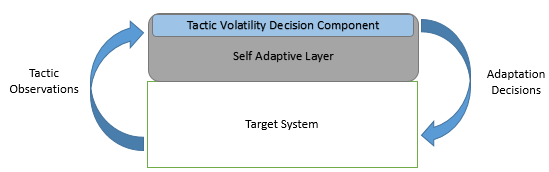
\includegraphics[scale=0.6]{images/TacticVolatilityProcess.png}
    \caption{Overview ofXXXX\dan{clean up image}}
    \label{fig:procOverview}
\end{figure}


\subsection{Evaluation Approach}

We will create and evaluate our tactic volatility based approach in several steps:

% Compare against baseline?
\begin{enumerate}[noitemsep]

%	In Full proposal should go into these steps much much more
	\item \textbf{\hl{Statistical Simulations}} We will first develop and evaluate our tactic volatility aware process using statistical simulators such as $R$. This evaluation will largely be used to provide initial feedback regarding approach. This efficient evaluation is imperative for building our initial models and subsequently evaluating any proposed approach, including evaluations against existing techniques. These simulations will also enable efficient evaluation under many hypothetical scenarios and settings. .

	\item \textbf{Existing Simulation Tools} After demonstrating the effectiveness of our approach in statistical simulators, we will next perform our evaluation using existing simulators. We will use popular simulation tools such as RUBiS\footnote{\url{http://rubis.ow2.org/}} and SWIM\footnote{\url{https://github.com/cps-sei/swim}}. These tools emulate intelligent web systems that collect data and make adaptive decisions. We will use these tools since they are well-known, and are able to simulate numerous real-world situations. We will also explore the use of other existing simulation tools as well. 

	\item \textbf{Custom-Built Simulators} To provide a more robust simulation environment, we will create several custom simulation tools. These will enable us to determine how our tactic volatility aware process works with large-scale data sets in various situations. There are several reasons for creating our own simulation tools including: I) The lack of existing options to simulate possible tactic volatility II) Do not simulate necessary events such as uncertainty\dan{add more reasons}. The PI is experienced in creating simulation tools for intelligent decision-making systems.\dan{Might be worth it to explain much more about these custom simulators. What will they mimic etc.....} % For the full proposal really build up this section 
           
	\item \textbf{Physical Devices} After our proposed method has demonstrated its effectiveness in several types of software simulations, we will then implement our decision-making process into several physical devices. These include single UAVs, robotic swarms, IOT devices, and a cloud-based system. simulation tools.\dan{add another few sentence to this. Provide confidence in our plan} 

\end{enumerate}

We will initially use existing data sets\footnote{\url{http://ita.ee.lbl.gov/}} for our simulations, but will use generated real-world data as it becomes available; especially from tests ran from our physical devices. We are well-suited to conduct this analysis due to: I) Our expertise in intelligent systems II) Cybersecurity expertise III) Access to drones and other physical resources.
    
       
       

% The Monitor-Analyze-Plan-Execute plus Knowledge (MAPE-K)~\cite{kephart2003vision} feedback loop is commonly used in self-adaptive systems. Our latency volatility approach will easily integrate into this MAPE-K loop in the `Analyze \& Plan' stage, as shown in Figure~\ref{fig:procOverview}.


% \begin{figure}[h]
% 	\centering
%     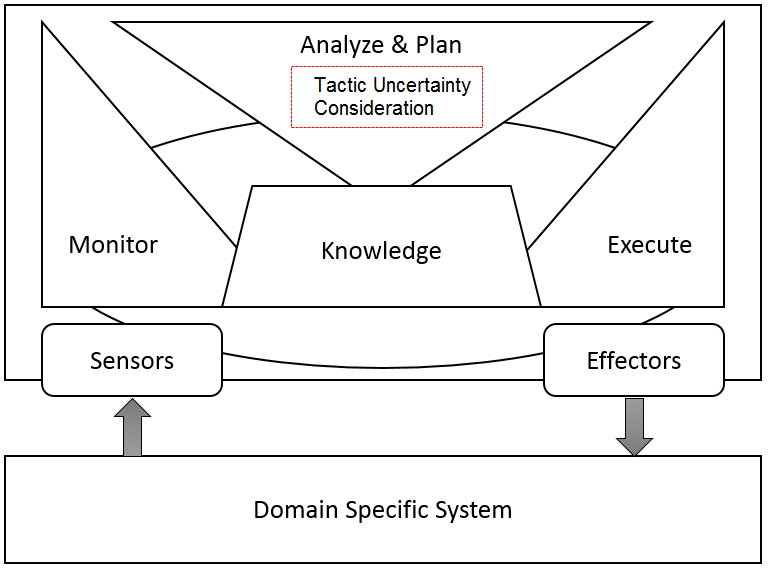
\includegraphics[scale=0.4]{images/mapek-red.png}
%     \caption{MAPE-K Self-Adaptation Loop With XXX Integrated in the `Analyze \& Plan' Stage\dan{clean up image}}
%     \label{fig:procOverview}
% \end{figure}



%% For the Technical approach should we describe some formulas a bit more?
%%%% For the full proposal we can go into more detail regarding the formula
% HOw will we compare the formulas against the baseline etc..... - What baseline will we use



\section{Technical Challenges}

%In this section the principal investigator answers questions such as, “What are the specific technologies to be developed?” or “What are the specific difficulties to be encountered?” It lists the technical hurdles that must be overcome to meet the technical objectives, identifying the ones that are the most important or the most difficult. This section should require one page at most. 





There are several technical challenges that must be overcome in both development and evaluation of our proposed work.


The first challenge to overcome is that uncertainty is difficult to plan for. Due to the inherit variable nature of uncertainty, it is challenging to incorporate into many decision-making models, and can be difficult to even test for. To address this challenge, we will use existing datasets\hl{finish....}


\todo{Simulating battlefield situations is hard}
\todo{How to decide the most appropriate utility}


% Create simulations
% Including in actual devices
% Uncertainty is ..... (cite some existing workds)
% Uncertainty by its very nature is unknown



% Where will we get our data

Simulating uncertainty is frequently a difficult challenge

%One is what does it mean to simulate uncertainty? Uncertainty could be because there is no way to know something because it changes all the time. In that case you’d be simulating the thing that changes. But uncertainty can also be about not knowing something that is knowable. So, how is that going to be simulated?



% Simulation Creation



% Physical Testing
The final stage of evaluating and demonstrating the impact of our findings will be to incorporate our improved decision-making process into physical devices, such as drones and IOT devices. We are confident in our abilities to address these challenges due to our expertise in software engineering, and the University's extensive drone research infrastructure. % DK: Add more to this





\section{Budget Summary}

The total budget is \$150K/yr for a total cost of \$450k for the three year project. Our budget will include: I) PhD Student support II) Equipment III) Travel support for collaborating DOD employees (who we already have a close relationship with), along with identified ONR collaborators. IV) We will also hire a DOD consultant to act as a technical advisor. PI Krutz has experience working with DOD agencies including researchers at the AFRL. A broad overview of our funding plan for each fiscal year is shown in Table~\ref{table:budget}.

% Change this a bit more for different agencies
 
%Co-PI Krutz will be working as 

% DK: Should the budget go up or down depending on year?

\begin{table}[h]
\begin{center}
\caption{Budget Summary}
\label{table:budget}

\begin{tabular}{ c | c | c }
			
  \textbf{Year 1} & \textbf{Year 2} & \textbf{Year 3}  \\   \hline
  150K & 150K & 150K \\
   \end{tabular}
  \end{center}
\end{table}






%\section{Relevance of Proposed Effort}
% Relevance of the proposed effort to the research areas described in Section II; relationship of the proposed work to current state of art.


% Describe current state of AI. Describe weakness in current solutions





% Regardless of the approach, proposed work should include what parts of the complex decision-making problem each of the componenht approaches is best suited to address

%DK: Not sure if this goes here




%\section{Technical Objective}
% Technical objective of the proposed effort;








%\section{Technical Approach}
% Technical approach that will be pursued to meet the objective;








%\section{Summary of Recent Work}
% A summary of recent relevant technical breakthroughs; and








\bibliographystyle{plain}
\bibliography{latency}

\end{document}


% ONR: https://www.onr.navy.mil/-/media/Files/Funding-Announcements/BAA/2018/N00014-18-S-B001.ashx
% Page limit– 5 pages. (pg 14)

% For ONR Only: Electronic (email) submissions should be sent to the
attention of the TPOC at: Email address of the TPOC, e.g., Jane.Doe@navy.mil. The subject line of the email shall read: “N00014-18-S-B0001” White Paper Submission”. Do not send ZIP files. Password protected files are discouraged.


%%%% ONR Solicitation Possibilities
%	


% https://www.rochester.edu/college/research/assets/pdf/LBA-DOD-101-UR.pdf - Good general resource on DOD funding and process

% 
